\documentclass[11pt, twocolumn]{article}
\usepackage{booktabs}
\usepackage{pdfpages}
\usepackage{siunitx}

\setlength{\parindent}{0pt}
\setlength{\parskip}{0.1in plus0.1in minus0.05in}


\sisetup{
  range-phrase	=	--		,
  range-units	=	brackets,
}

\begin{document}

\title{HF QRP Cheat Sheet}
\author{Steve Herrin (AG6VF)}
\date{}
\maketitle
\newpage



\section{Band Plan}


\subsection{160 meters (\SIrange{1.8}{2.0}{\MHz})}
Long-distance propagation at night. Better in the winter.

For SSB, use LSB.
\begin{center}
  \begin{tabular}{S l}
    {Frequency (\si{\MHz})}	&	Mode(s)			\\
    \midrule
    \numrange{1.800}{2.000}	&	CW				\\
    \numrange{1.800}{1.810}	&	Digital			\\
    \num{1.810}				&	CW Calling		\\
    \num{1.818}				&	CW Calling		\\
    \numrange{1.843}{2.000}	&	SSB, SSTV, Other\\
    \num{1.910}				&	SSB Calling		\\
    \numrange{1.995}{2.000}	&	Experimental	\\
    \numrange{1.999}{2.000}	&	Beacons			\\
  \end{tabular}
\end{center}


\subsection{80 meters (\SIrange{3.5}{4.0}{\MHz})}
Long-distance propagation at night. Better in the winter.
Longer distances than \SI{160}{\m}. Reliable.

For SSB, use LSB.
\begin{center}
  \begin{tabular}{S l}
    {Frequency (\si{\MHz})}	&	Mode(s)					\\
    \midrule
    \num{3.560}				&	CW Calling				\\
    \num{3.590}				&	RTTY/Data DX			\\
    \numrange{3.570}{3.600}	&	RTTY/Data				\\
    \num{3.710}				&	CW Calling (Novice) 	\\
    \num{3.711}				&	CW Calling (Novice)		\\
    \numrange{3.790}{3.800}	&	DX Window				\\
    \num{3.845}				&	SSTV					\\
    \num{3.885}				&	AM Calling				\\
  \end{tabular}
\end{center}


\subsection{60 meters (\SI{5}{\MHz} channels)}
Similar to \SI{80}{\m} and \SI{40}{m}. 

Only allowed on 5 channels. Only one signal at a time is permitted
on a channel. Maximum power \SI{100}{\W} PEP.

USB is limited to \SI{2.8}{\kHz}.

CW and digital must be centered \SI{1.5}{\kHz} above the frequencies shown.

\begin{center}
  \begin{tabular}{S l}
    {Frequency (\si{\MHz})}	&	Mode(s)					\\
    \midrule
    \num{5.3305}			&	USB and CW/RTTY/Data	\\
    \num{5.3465}			&	USB and CW/RTTY/Data	\\
    \num{5.3570}			&	USB and CW/RTTY/Data	\\
    \num{5.3715}			&	USB and CW/RTTY/Data	\\
    \num{5.4035}			&	USB and CW/RTTY/Data	\\
  \end{tabular}
\end{center}


\subsection{40 meters (\SIrange{7.0}{7.3}{\MHz})}
During the summer, \SIrange{500}{700}{\km} range during the day,
and \SI{1500}{\km} range during at night. Better in the winter.

For SSB, use LSB.
\begin{center}
  \begin{tabular}{l l}
    {Frequency (\si{\MHz})}	&	Mode(s)					\\
    \midrule
    \num{7.040}				&	CW Calling				\\
    \num{7.040}				&	RTTY/Data DX			\\
    \numrange{7.080}{7.125}	&	RTTY/Data				\\
    \num{7.110}				&	CW Calling (Novice)		\\
    \num{7.171}				&	SSTV					\\
    \num{7.285}				&	SSB Calling				\\
    \num{7.290}				&	AM Calling				\\
  \end{tabular}
\end{center}

\subsection{30 meters (\SIrange{10.1}{10.15}{\MHz})}
Like \SI{40}{m}, but slightly longer propagation.

Can only be used for CW and RTTY.
\begin{center}
  \begin{tabular}{l l}
    {Frequency (\si{\MHz})}		&	Mode(s)			\\
    \midrule
    \num{10.106}				&	CW Calling		\\
    \num{10.116}				&	CW Calling		\\
    \numrange{10.130}{10.140}	&	RTTY			\\
    \numrange{10.140}{10.150}	&	Packet			\\
  \end{tabular}
\end{center}


\subsection{20 meters (\SIrange{14.0}{14.35}{\MHz})}
Around-the-world propagation, at peak solar cycle. Not
useful for short ranges (a few \SI{100}{\km}).

For SSB, use USB.
\begin{center}
  \begin{tabular}{l l}
    {Frequency (\si{\MHz})}		&	Mode(s)			\\
    \midrule
    \num{14.060}				&	CW Calling		\\
    \numrange{14.070}{14.095}	&	RTTY			\\
    \numrange{14.0950}{14.0995}	&	Packet			\\
    \num{14.100}				&	Beacons			\\
    \numrange{14.1005}{14.1120}	&	Packet			\\
    \num{14.230}				&	SSTV			\\
    \num{14.285}				&	SSB Calling		\\
    \num{14.286}				&	AM Calling		\\
  \end{tabular}
\end{center}


\subsection{17 meters (\SIrange{18.068}{18.168}{\MHz})}
Similar to \SI{20}{m}.

For SSB, use USB.
\begin{center}
  \begin{tabular}{l l}
    {Frequency (\si{\MHz})}			&	Mode(s)		\\
    \midrule
    \num{18.069}					&	CW Calling	\\
    \num{18.096}					&	CW Calling	\\
    \numrange{18.100}{18.105}		&	RTTY		\\
    \numrange{18.105}{18.110}		&	Packet		\\
    \num{18.130}					&	SSB Calling	\\
  \end{tabular}
\end{center}


\subsection{15 meters (\SIrange{21.000}{21.450}{\MHz})}
Similar to \SI{20}{m}, but less reliable and even more influenced
by the solar cycle.

For SSB, use USB.
\begin{center}
  \begin{tabular}{l l}
    {Frequency (\si{\MHz})}		&	Mode(s)				\\
    \midrule
    \num{21.060}				&	CW Calling			\\
    \numrange{21.070}{21.110}	&	RTTY/Data			\\
    \num{21.110}				&	CW Calling (Novice)	\\
    \num{21.340}				&	SSTV				\\
    \num{21.385}				&	SSB Calling			\\
  \end{tabular}
\end{center}


\subsection{12 meters (\SIrange{24.89}{24.99}{\MHz})}
Even more strongly influenced by the solar cycle than \SI{15}{m}.

For SSB, use USB.
\begin{center}
  \begin{tabular}{l l}
    {Frequency (\si{\MHz})}			&	Mode(s)		\\
    \midrule
    \num{24.906}					&	CW Calling	\\
    \numrange{24.920}{24.925}		&	RTTY		\\
    \numrange{24.925}{24.930}		&	Packet		\\
    \num{24.956}					&	SSB Calling	\\
  \end{tabular}
\end{center}


\subsection{10 meters (\SIrange{28.0}{29.7}{\MHz})}
Most influenced by the solar cycle. Good for DX and QRP when
the conditions are right.

For SSB, use USB.
\begin{center}
  \begin{tabular}{l l}
    {Frequency (\si{\MHz})}			&	Mode(s)				\\
    \midrule
    \numrange{28.000}{28.070}		&	CW					\\
    \num{28.060}					&	CW Calling			\\
    \numrange{28.070}{28.150}		&	RTTY				\\
    \num{28.110}					&	CW Calling (Novice)	\\
    \numrange{28.150}{28.190}		&	CW					\\
    \numrange{28.200}{28.300}		&	Beacons				\\
    \numrange{28.300}{29.300}		&	Phone				\\
    \num{28.680}					&	SSTV				\\
    \num{28.885}					&	SSB Calling			\\
    \numrange{29.000}{29.200}		&	AM					\\
    \numrange{29.300}{29.510}		&	Satellites			\\
    \numrange{29.520}{29.590}		&	Repeater Inputs		\\
    \num{29.600}					&	FM					\\
    \numrange{29.610}{29.700}		&	Repeater Outputs	\\
  \end{tabular}
\end{center}


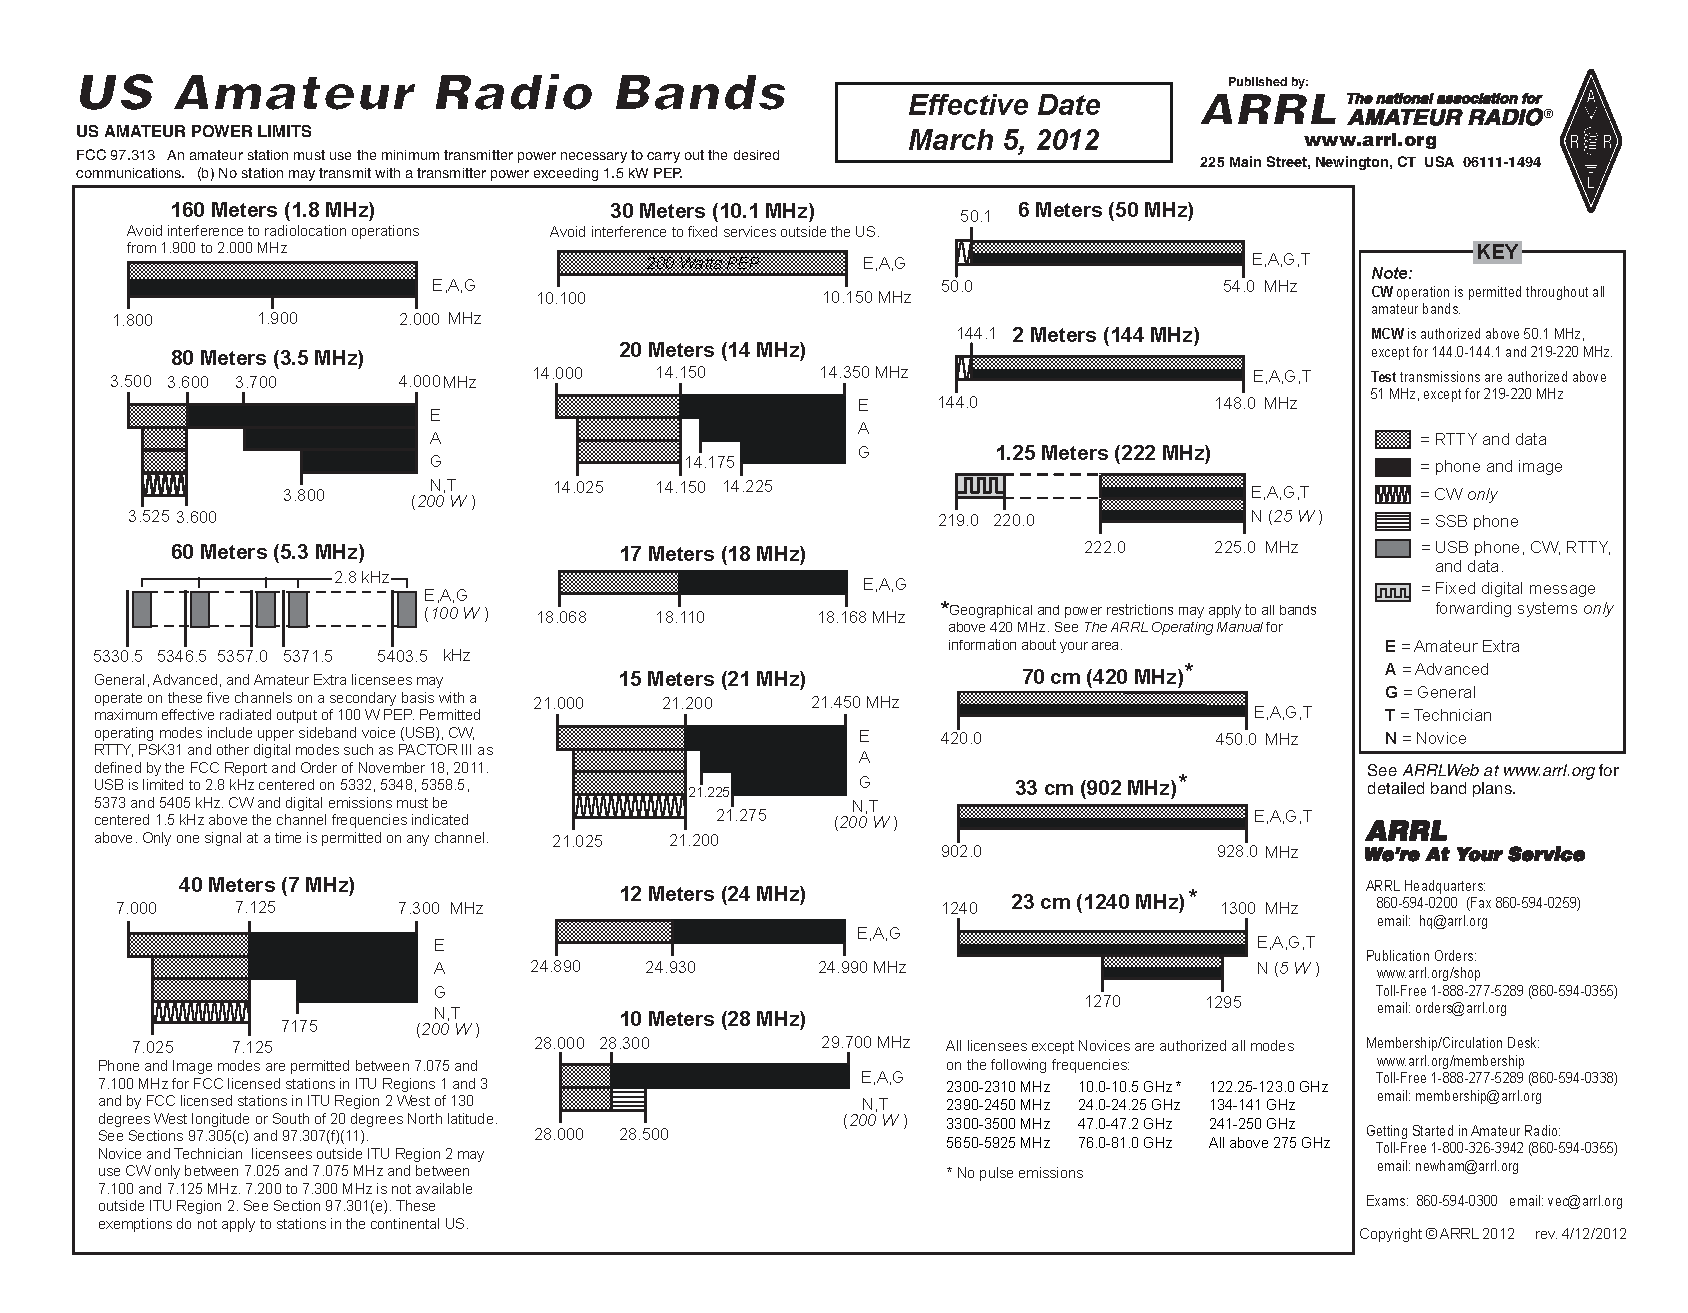
\includepdf[landscape=true]{hambands_bw.pdf}



\section{WWV}
WWV is operated by NIST and broadcasts official U.S.\ Government frequency and time signals.
\begin{center}
  \begin{tabular}{S}
    {Frequency (\si{\MHz})} \\
    \midrule
    2.5	\\
    5.0	\\
    10.0	\\
    15.0	\\
    20.0	\\
  \end{tabular}
\end{center}

\end{document}
